\documentclass[main.tex]{subfiles}
\begin{document}

\section{iOS Development}


\subsection{Building an iOS application}

There are several things that are needed to build a working iOS application. iOS applications work using the Model View Controller (MVC) design pattern. This attempts to separate the interface of the application (views) from the inner workings and data stored (model) with communication between these two components being moderated by a separate class (controller). Each class created in an MVC application should ideally fall under one of these categories. 

\subsubsection{Model}

In an MVC application, the model is designed to encapsulate the problem-domain and internal logic of the application. That is, it is responsible for generating, storing and processing the information that is related to the application. It is also responsible for any data access including web access and communicating with an external storage system such as a database. A simple diagram of an MVC architecture is shown in image \ref{MVC}. The application logic and data access sections of the model should not be aware of the inner workings of each other in order to provide flexibility when changing the type of data storage or the application logic. 

\subsubsection{View}

The view is the part of the application that shows the various components and data on the screen for the user to see. It is also responsible for providing the necessary components that can allow the user to interact with the application. The view is additionally responsible for presenting any data given to it in a human readable way, such as presenting it in a graph or pie chart or in a listed table. In iOS, views are created with the use of the storyboard feature that is described in more detail below.

\subsubsection{Controller}

The controller is the final piece of the application that links the views to the model. The controller is primarily what the user interacts with whenever they interact with the application. While the view is responsible for showing any inputs such as buttons and text fields, it is the view controller that converts these into commands which are passed down to the model. Similarly, any information returned by the model is converted into the proper format by the controller and given to proper view in order to show. In a way, the controller is the glue that binds both the views and the models together and there should be no communication between the two that does not go through the controller at some point.

\begin{figure}[]
\centering
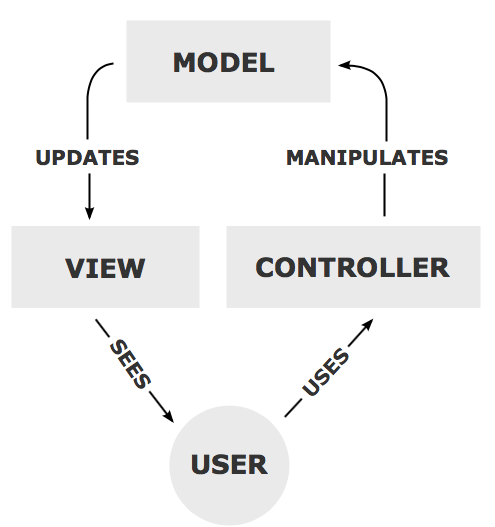
\includegraphics[width=0.5\textwidth]{images-implementation/MVCLayout.png}
\label{MVC}
\caption{Diagram showing a simple flow chart of an MVC application. Image obtained from \cite{mvc}}
\end{figure}


\subsection{Storyboards}
One of the other most important concepts in iOS development is storyboards. Storyboards work as a view designer and transitioning controller between different views. They provide the hooks through which a controller can process inputs and tell the views what and how to interact with the user. Storyboards as an iOS specific feature and typically require the use of Apples Xcode development platform to view and edit. However Xamarin has their own version of the storyboard editor that provides some support for C\# based coding and is easier to use to hook visual components into the C\# code in the view controller.

\subsection{APIs}
iOS provides a vast host of APIs that are ideal for a large number of tasks such as displaying information and resources as well as accessing on-device data such as accelerometer and gyroscope data. Apple’s original iOS APIs are available as C\# libraries under the Xamarin framework and are very similar in structure and usage to the original Objective-C and Swift versions. These APIs are designed to be as easy to implement as possible and this was really seen during development when compared to Android development as certain functionality and sensor readings was seen to be much more easily accessible in iOS. Additionally, much of the functionality follows a very strict hierarchical inheritance structure which lends its hand to many scenarios such as creating a complex view. All iOS visual components inherit from the UIView class, of which a component of this is a collection of UIView named subviews which are rendered within relation to the parent UIView. This effectively allows a hierarchical structure of UIViews which can be rendered and set dynamically. UIView classes also have the added functionality to automatically redraw whenever a change is made with them, as long as this call is made on the main UI thread. This structuring, alongside the simplistic nature of the components and their ease of creation, modification and rendering, makes it incredibly easy to create complex applications from just a few simple boiler plate components.

\subsection{Development}

Our development for an iOS application started with creating a simple blank Xamarin cross platform solution for android and iOS. This provides 3 separate projects in which we can work with. There is 1 project each for the different mobile platforms and a 3rd project that acts as the standalone shared code that can be accessed by both iOS and Android. Due to the nature of this, the shared code project must be written independently from any specific platform and cannot use or rely on libraries or functionality that are specific to a single platform.

\subsubsection{Storyboard and Interface}
We start off with a single storyboard for iOS simply titled main.storyboard. From here, we built the visual end of the iOS application and determined how many different screens (views) we were going to have and how to transition between them. We decided to only go with one storyboard since there were not going to be many screens and the transitions between them would be simple and would use pre-made segues (transitions in iOS). We start simply with a Navigation Controller. A Navigation Controller is a class that is responsible for controlling a hierarchical navigation of different screens as seen in many native iOS applications.

\begin{figure}[]
\centering
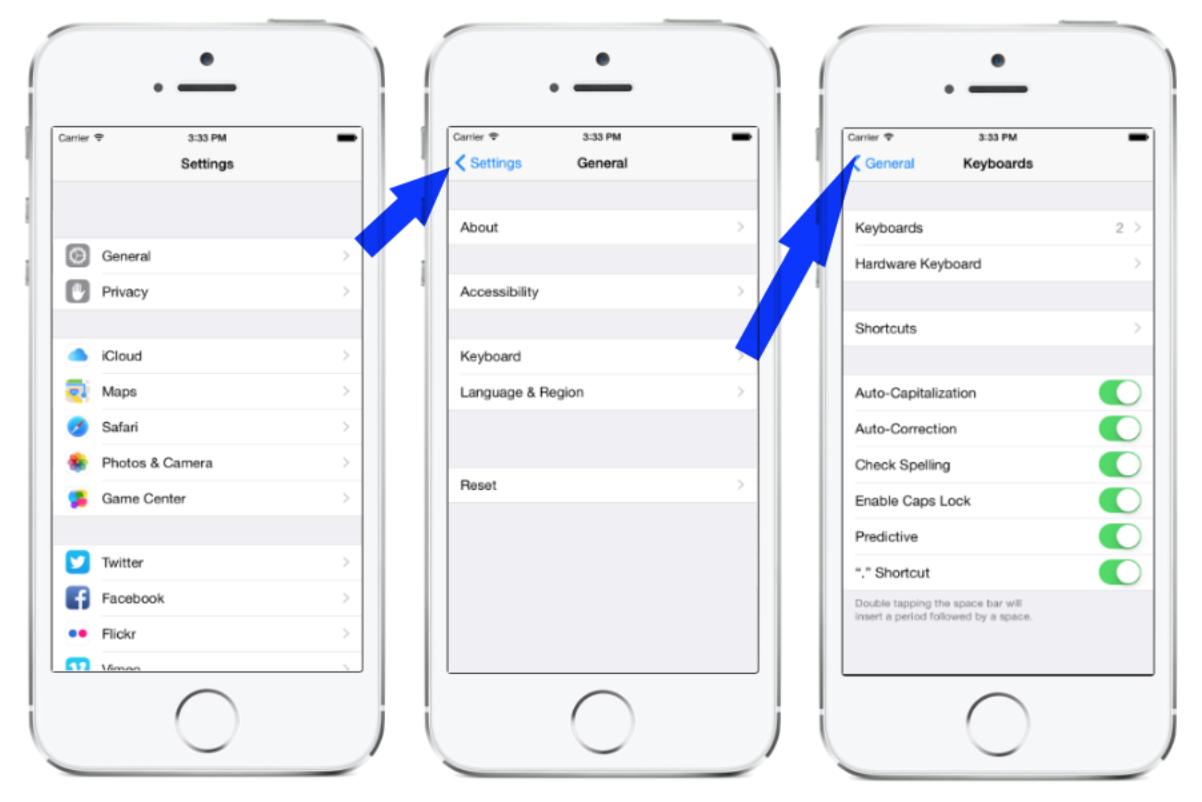
\includegraphics[width=0.5\textwidth]{images-implementation/NavigationController.png}
\label{NavigationController}
\caption{Image showing the workings of the Navigation Controller component in iOS .Image obtained from \cite{iosnavigxtioncontroller}.}
\end{figure}

A Navigation Controller is able to keep track of the visited screens and the path that the user has taken through them and allows the user to back-track through the application. We initially use this to create an options screen which could linked to from a button on the title bar of the main screen shown in image \ref{initStoryboard}. The Navigation Controller then automatically creates the back button on the options page. This can allow for a complex hierarchical structure that is easily controlled and changed.

\begin{figure}[]
\centering
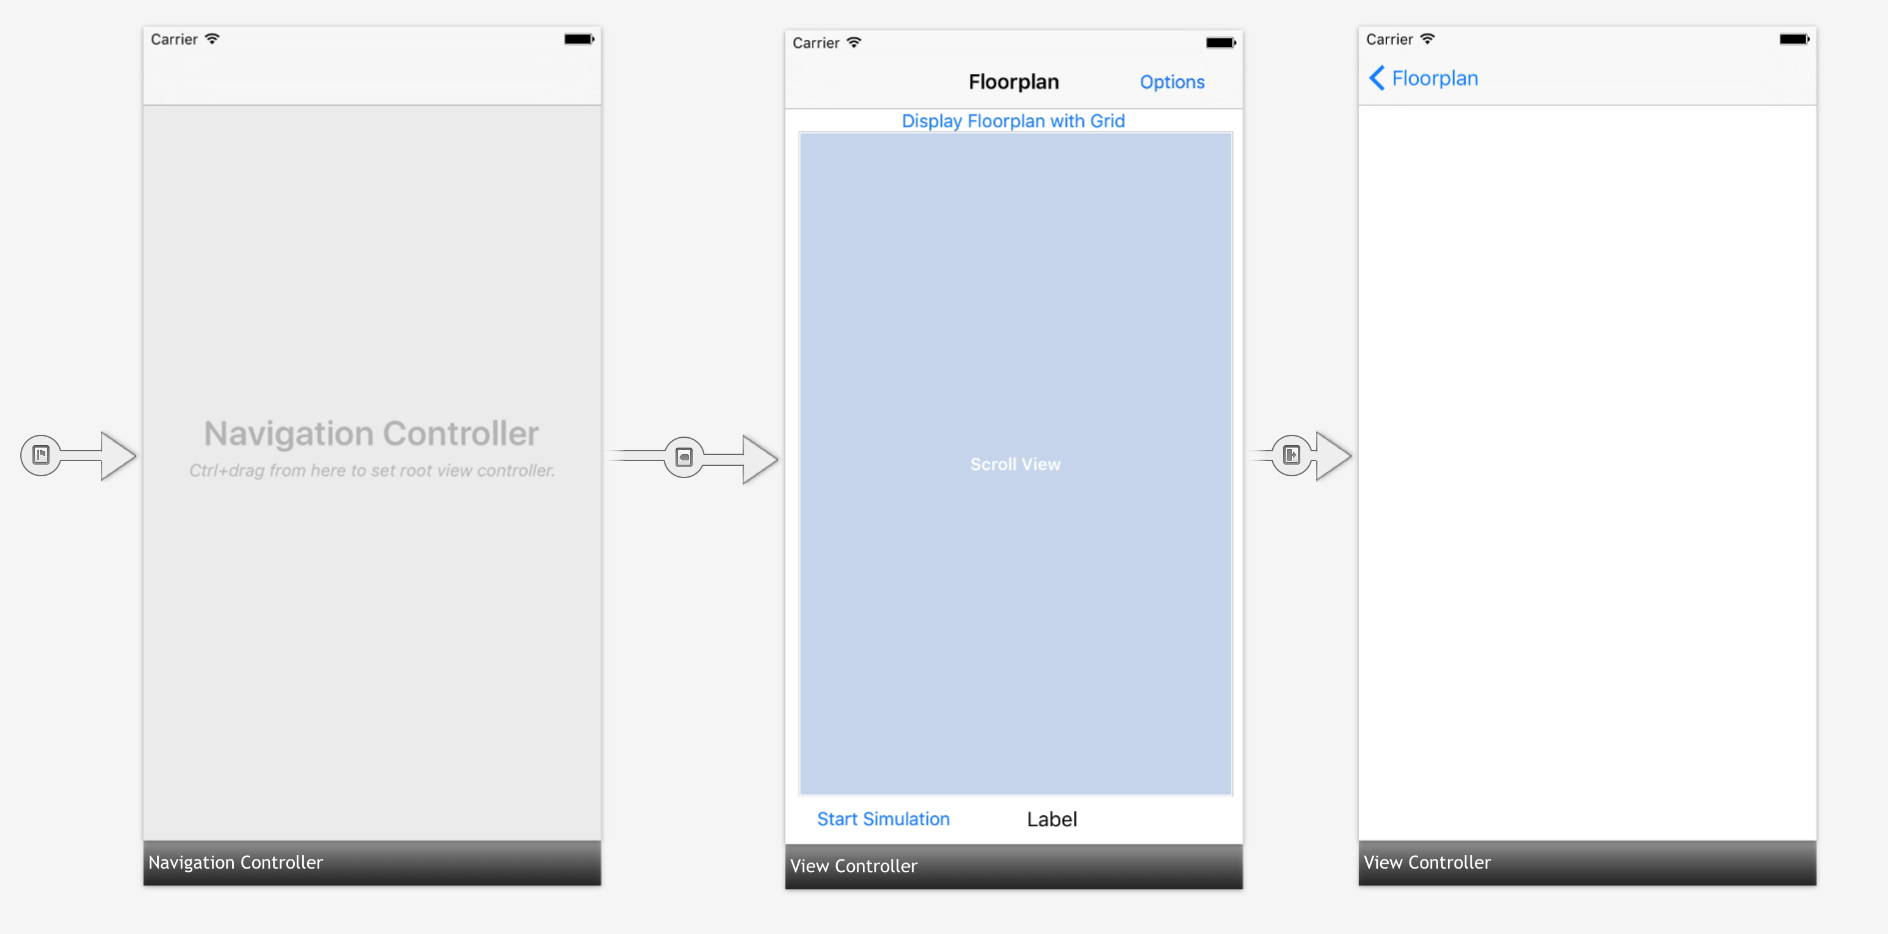
\includegraphics[width=0.5\textwidth]{images-implementation/InitialStoryboard.png}
\label{initStoryboard}
\caption{Screenshot showing a early design for the main storyboard. The Navigation Controller and its derived navigation controls can be seen in the title bars for the different screens shown.}
\end{figure}

The main map view was implemented using a UIScrollView class. This would allow us to show an image which could be panned and zoomed, as well as respond to additional gestures on top. Since UIScrollView is able to display any UIView class, this allows us to display many views that will pan and zoom together by wrapping them in a UIView wrapper. Since the map images and other components were going to be loaded dynamically, they had to be set manually in the view controller rather than in the storyboard editor. To achieve this, we needed a hook to the scroll view in order to set the contents dynamically in the view controller. This is a very simple procedure in Xamarin and simply involves giving the component a name. Doing so will create a hook in the ViewController.designer.cs class which is a partial class of ViewController.cs. This allows us to reference the scroll view and set up the contents and properties accordingly from within the View Controller. This is described in detail in the View Controller section.

We decided to implement a search functionality to allow users to search for the room they are looking for. This would then allow them to select whether to set their location to that room, or to set that room as a destination for navigating to. To do this, we added 2 new components to the main view of the application; a search bar and a search results/prediction table. These components can be seen as storyboard components in image \ref{IOSRoomSearchInStoryboard}. As part of our implementation for representing the floor plan, we also had a list of all the rooms contained by the map. This was implemented using a custom controller called CustomSearchController.cs and the search bar and table view were hooked into the View Controller in the same way that the scroll view was. This class would take references to the search bar and table view components, as well as a list of the rooms obtained from the floor resources. All logic pertaining to the search functionality was then performed in this class and other classes referenced by it, this allowed us to separate out certain functionalities from the main view controller. A working version of the room search functionality can be seen in image \ref{IOSRoomSearchInApp}.

\begin{figure}[]
\centering
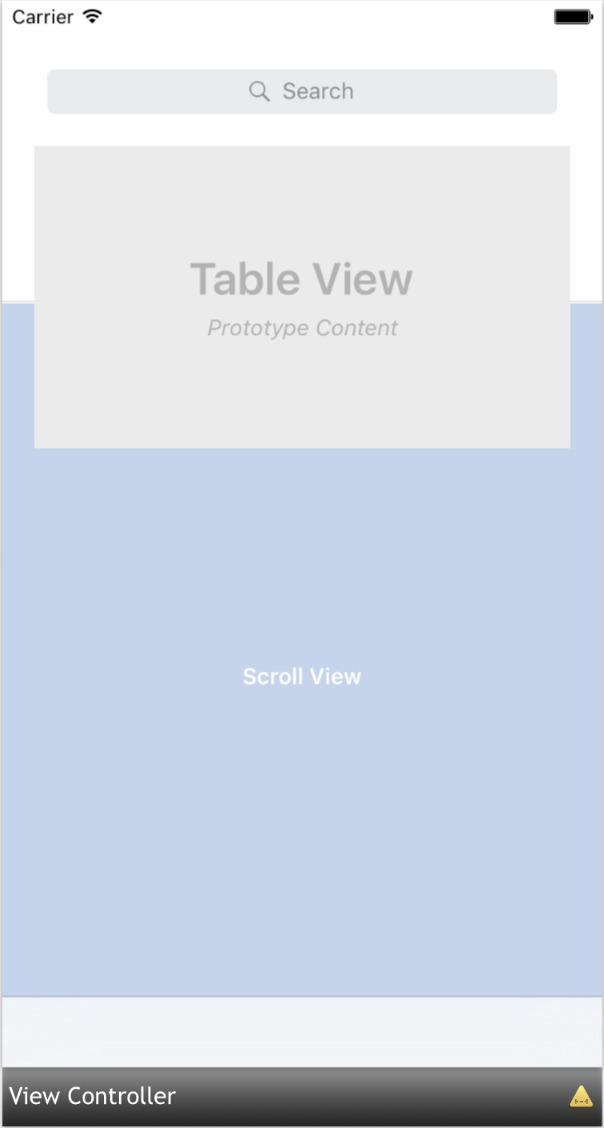
\includegraphics[width=0.5\textwidth]{images-implementation/IOSRoomSearchInStoryboard.png}
\label{IOSRoomSearchInStoryboard}
\caption{Screenshot showing how the search bar and result/prediction table are shown in the main storyboard.}
\end{figure}


\begin{figure}[]
\centering
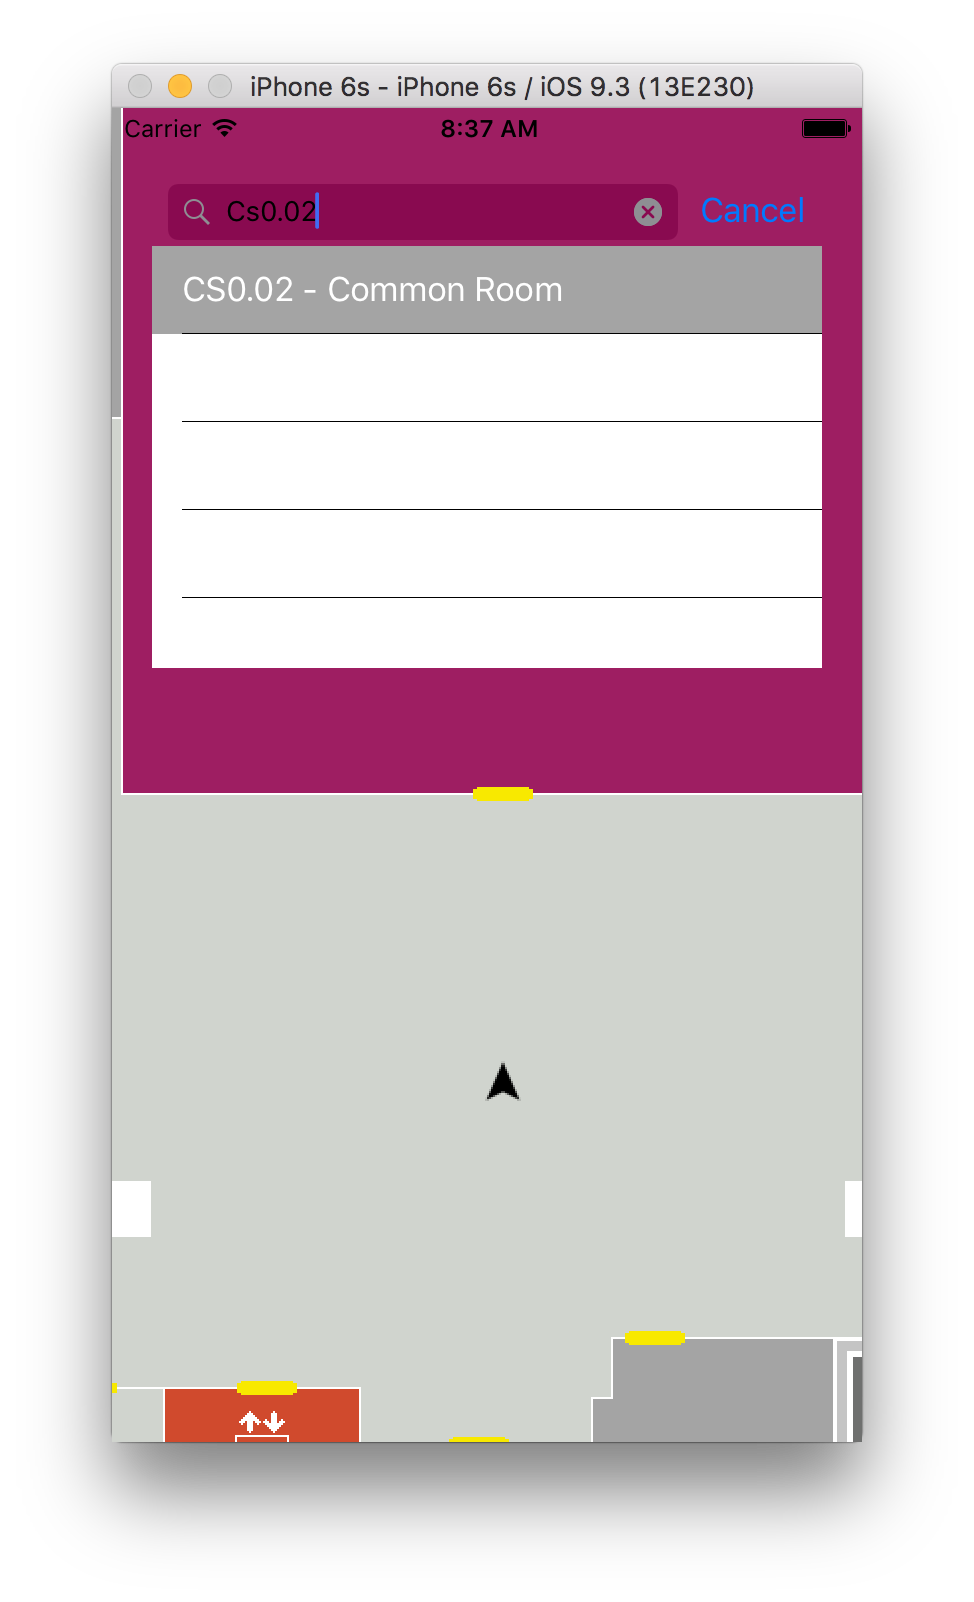
\includegraphics[width=0.5\textwidth]{images-implementation/IOSRoomSearchInApp.png}
\label{IOSRoomSearchInApp}
\caption{Screenshot showing how the search bar and result/prediction table are shown in the application.}
\end{figure}


 




\subsubsection{View Controller}
The ViewController.cs file is where the majority of the iOS specific code is kept. It is responsible for delegating all communication between the view components and the model of the application which was kept in the shared code project. It was also responsible for assigning many of the dynamic variables and properties of the view components that could not be simply created using the storyboard editor. Because of this, the view controller class is one of the longest, most feature heavy classes that is present in the application. One of the primary goals at the beginning of the project was to be able to get a simple view of a map on the screen that could be panned and zoomed by the user. We achieved this primarily with the use of a UIScrollView class. The initial scroll view component was placed using the storyboard editor, however since we wanted the image displayed to be able to be loaded dynamically to facilitate changing maps, we could not set the contents or any derived properties (such as content width and height) from the storyboard editor and instead had to elicit the use of the view controller class. An object hook was placed so that we could refer to the scroll view from inside the view controller and the following code was used to import and display the map.
\begin{lstlisting}
floorplanImageNoGrid = 
	UIImage.FromBundle("Images/FinalDcsFloor1.png");
floorplanImageView.Image = floorplanImageNoGrid

floorplanScrollView.AddSubview(floorplanImageView);
floorplanScrollView.ContentSize = floorplanImageNoGrid.Size;
floorplanScrollView.ViewForZoomingInScrollView += 
	(UIScrollView sv) => { return floorplanImageView; };
\end{lstlisting}
The first 2 lines of this code segment simply loads the proper map image from the applications resources and assigns it to a UIImageView class in order to be able to interact with other UIView classes. The 3rd line then adds this subview to the scroll view which is already set to display on the screen. The 4th and 5th lines are included in order for panning and zooming to work correctly. This simply set the contained size of the scroll view to be equal to that of the image view and the scroll view is told to zoom the image view when pinch-to-zoom gestures are registered. This code segment was included as a simple example to show how easy it is to include and manipulate visual components with ease in iOS. While this is a simple example, the main concepts of a hierarchical architecture of UIViews will remain for the remainder of this section. It is important to note that a UIView can contain more that one subview.

The next step in creating a usable navigation app is to be able to draw things on the map such as the user's location and the path to their destination. Here we can utilise the structuring of UIViews by creating a container view. This is an effectively invisible view that essentially encapsulates 2 or more subviews into one container that can be acted upon and changed as a single entity. By creating a container view with the map image and a user's location arrow image as subviews, we can instruct the scroll view to act upon the container view instead of either of the subviews. This results in the scrollview being able to pan and zoom both views simultaneously to create seemingly one picture. 

\begin{lstlisting}
container.AddSubview(floorplanImageView);
container.AddSubview(userLocationArrow);
container.SizeToFit();

floorplanScrollView.ContentSize = container.Size;
floorplanScrollView.ViewForZoomingInScrollView += 
	(UIScrollView sv) => { return container; };
\end{lstlisting}
While this works nicely, we noticed that on many existing mapping applications such as Google and Apple Maps, the user location arrow did not scale with the map when zooming. Instead it stayed at a constant size and simply stayed to reflect the correct location. This was unfortunately not as simple a change as you might expect. By changing the floowplanScrollView.ViewForZoomingInScrollView property to return just the map UIImageView, we ran into the problem that the user location arrow could not distinguish between the absolute coordinated on the map and the relative coordinates to the container view. This effectively meant that as the view was scrolled in and out, the relative position of the arrow on the map would increase and the map images coordinate space was compressed. The easiest solution we could find to this problem was to manually recalculate and modify the location arrow coordinates in relation to the zoom factor of the scroll view.


[image of incorrect location arrow zooming]
[image of correct location arrow zooming]

\subsubsection{Paths}

The second part that needed drawing over the main map was the actual path to the user's destination. iOS supplied a useful CGPath component that could draw a customised line between a set of points on a 2D space. However, in order to be compatible with the other UIView based components, we had to create a custom PathView.cs class that would act as a wrapper to the CGPath class. This class would be responsible for drawing the path and ensuring it remains consistent with the map image during zooming. It would also contain additional methods for encapsulating the CGPath object from the outside and for adding and getting points on the path in an abstracted way. 

In order to interact with the map, we implemented a gesture recogniser on the scroll view. This allows for a long tap and hold on any part of the image and would result in a popup that would allow the user to set the point as either a start or and end point for a path. Setting a start location would move the user to that particular point, while setting an end location would attempt to draw a path from the user to the destination. Creating this was fairly simple and simply required the use of the UIAlertController class which allowed us to create iOS style alerts with customisable options. An image for a preliminary options sheet is shown in image \ref{IOSAlertSheet} and the code is shown below.

\begin{figure}[]
\centering
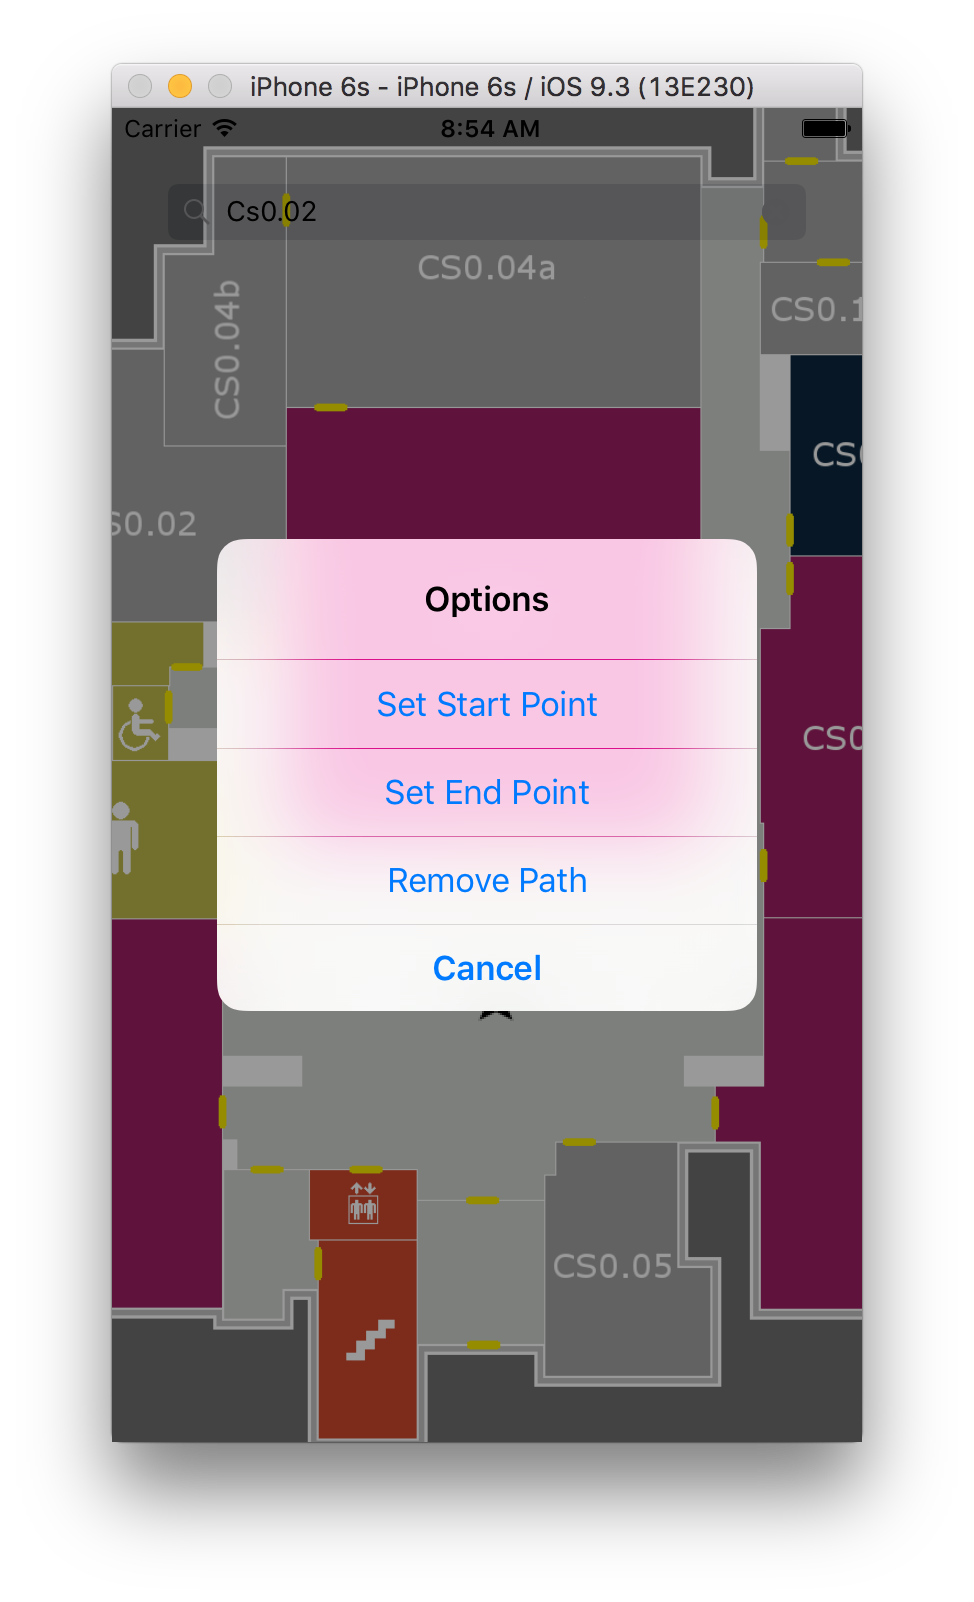
\includegraphics[width=0.5\textwidth]{images-implementation/IOSAlertSheet.png}
\label{IOSAlertSheet}
\caption{Screenshot showing the iOS alert sheet that would show when long pressing an area on the map.}
\end{figure}

\begin{lstlisting}
// Create a new Alert Controller
UIAlertController actionSheetAlert = UIAlertController.Create(
	"Options", 
	null, 
	UIAlertControllerStyle.Alert
);

// Add Actions
actionSheetAlert.AddAction(
	UIAlertAction.Create("Cancel",
	UIAlertActionStyle.Cancel, 
	null));
actionSheetAlert.AddAction(
	UIAlertAction.Create("Set Start Point",
	UIAlertActionStyle.Default, 
	(action) => setStartPoint(tapX, tapY)));
actionSheetAlert.AddAction(
	UIAlertAction.Create("Set End Point",
	UIAlertActionStyle.Default, 
	(action) => setEndPoint(tapX, tapY)));
\end{lstlisting}

\subsubsection{Getting Sensor Values}
One of the crucial aspects required for the step detector and wall collision classes to work was various device sensor readings. These included heading information and accelerometer and gyroscope values. Since these classes were designed and written as shared code to be utilised by both iOS and Android, they could not directly access these sensor readings themselves and instead had to implement methods for receiving these from the correct native projects. As such, sensor readings were the responsibility of the native projects to collect and manipulate into the correct format required by the step detector and wall collision classes. Retrieving sensor readings in iOS is fairly simple and many similar sensor readings are nicely encapsulated into easy to understand objects. Additionally, the Xamarin iOS framework makes use of the functional paradigm support of C\# in order to simplify the process of receiving updated sensor values. C\# is able to handle functions as first order variables, and as such, they can be easily passed into functions as arguments and can be dynamically run by variable name. This allows us to pass our handler functions into the sensor managers, that is, the code that will be run whenever a new set of updated values is provided. This allows easy encapsulation and purity of the sensor managers and a relatively simple solution to retrieving updated values, an issue that could potentially require a much more complex solution with other languages. To demonstrate this, we will show how accelerometer readings, which will be crucial for step detection, are taken on an iOS device using Xamarin and C\#. The method definition for retrieving accelerometer values is 
\begin{lstlisting}
CMMotionManager.StartAccelerometerUpdates(
	NSOperationQueue queue, 
	CMAccelerometerHandler handler
);
\end{lstlisting}
The important argument here is the CMAccelerometerHandler handler. This is where the method that is called whenever the accelerometer values are updated. The CMAccelerometerHandler referenced here is a delegate type. A delegate is a special keyword used by C\# to specify a method definition without actually specifying any actual body to the method. The declaration for CMAccelerometerHandler is shown below.
\begin{lstlisting}
public delegate void CMAccelerometerHandler (
	CMAccelerometerData data, 
	NSError error
);
\end{lstlisting}
What this declaration does is define a type of method CMAccelerometerHandler that takes those two particular arguments. Now any event that is created with the type CMAccelerometerHandler will require its subscriber methods to also implement this same declaration. This ensures that the correct arguments can be passed into the subscriber methods when the event is called. Shown below is the implementation used in our application for retrieving accelerometer values and passing them into the step detector class. In this example, we make use of an anonymous lambda function instead of declaring a full named method. As such, this lambda function has the same declaration as the CMAccelerometerHandler delegate.
\begin{lstlisting}
motionManager.StartAccelerometerUpdates(
	NSOperationQueue.CurrentQueue,
	(data, error) =>
	{
		accelX = data.Acceleration.X*9.8;
		accelY = data.Acceleration.Y*9.8;
		accelZ = Math.Sqrt(Math.Pow(accelX, 2) + 
			  Math.Pow(accelY, 2) + 
			  Math.Pow(data.Acceleration.Z*9.8, 2));

		col.PassSensorReadings(
			CollisionSensorType.Accelometer, 
			accelX, accelY, accelZ);
	});
\end{lstlisting}

The other sensor reading that was crucial for accurate plotting and to understanding where the user was on the map, was the device’s heading. There are a few methods that can be used to generate this information on iOS and several ways to represent it. Gyroscope readings from CMMotionManager, (same manager as accelerometer values,) we can obtain the instantaneous rotational velocity in any one of the 3 axis which can be turned into a relative heading, that is, the device rotated 15\textdegree counterclockwise. This however required knowledge of the initial heading in order to be able to properly estimate the heading of the device in relation to a map. Alternatively, through the use of CLLocationManager, we can obtain an estimation of the absolute heading of the device, (North, South, East, West). This measure is predominantly taken by the magnetometer sensor but may potentially be aided by other sensors such as the gyroscope. CLLocationManager utilises events in C\# in order to provide updated values for the heading. An event in C\# follows the pub-sub design pattern where various subscriber classes can subscribe a particular method they contain onto an event defined in another class, or in itself potentially. When the event’s owner class calls the event, each of the subscribed methods will be called, with any parameters to the event being passed into them. The heading values were provided to us in degrees with 0 representing North. This was quickly converted to radians to aid with calculations further down the line, and the new updated value was fed into the wall collision class.

\subsubsection{Path Smoothing}

The paths returned by the Dijkstra algorithm implementation usually quite jagged and not appealing visually. They also would not present a coherent path for the user to follow. This was a natural by-product of the grid based graph as can be seen within figure ~\ref{fig:jaggedPath}. Path smoothing was therefore implemented in order to create more logical and visually appealing paths.

\begin{figure}[]
\center
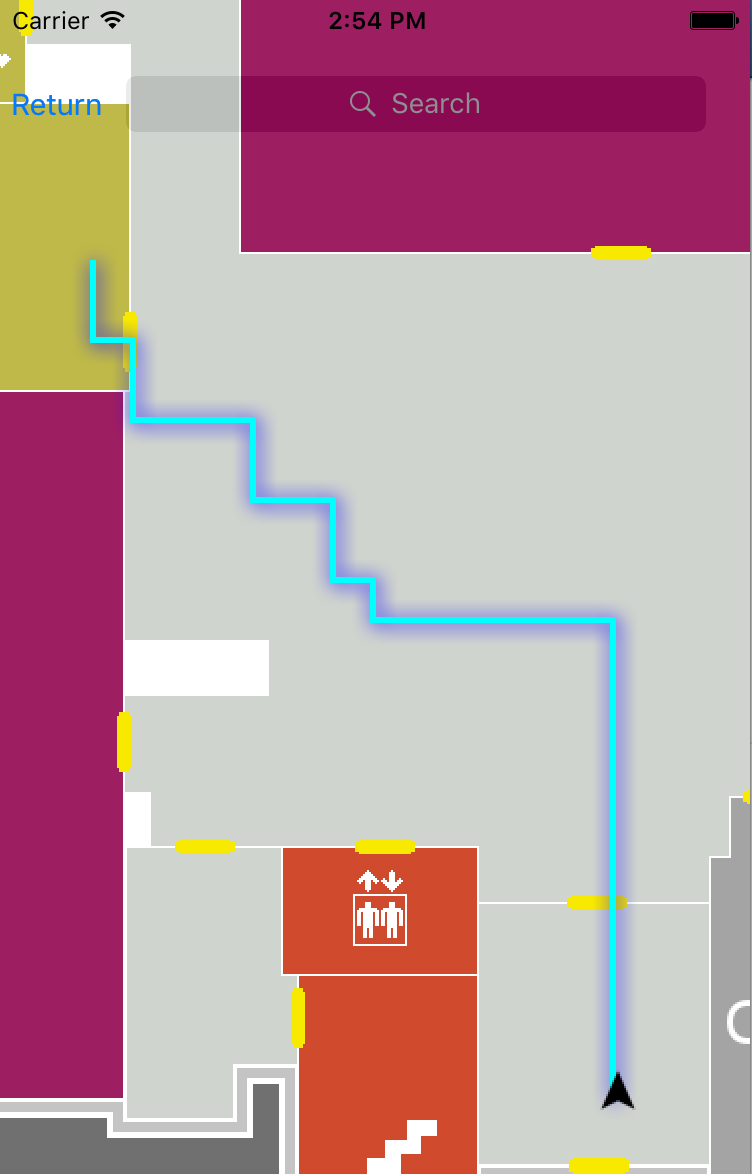
\includegraphics[width=0.5\textwidth]{images/jaggedPath.png}
\caption{Path displayed without path smoothing.}
\label{fig:jaggedPath}
\end{figure}


This made use of the previously mentioned wallCheck() method, which would take a line between two points and check whether it intersects with a wall within the floor plan image. In order to smooth the path, the algorithm first sets the initial point as the start point. Subsequent points are then iterated over and marked as end points. If a line between the set start and end points is shown to pass through a wall at any point, this end point is made the new start point, and the line between the previous start and end points is added to the new smoothed path. Repeating this process until all nodes on the path have been iterated over creates a smoothed path that maximises the spaces between bends in the path. The effects of this smoothing technique are shown within figure ~\ref{fig:smoothPath}.

\begin{figure}[]
\center
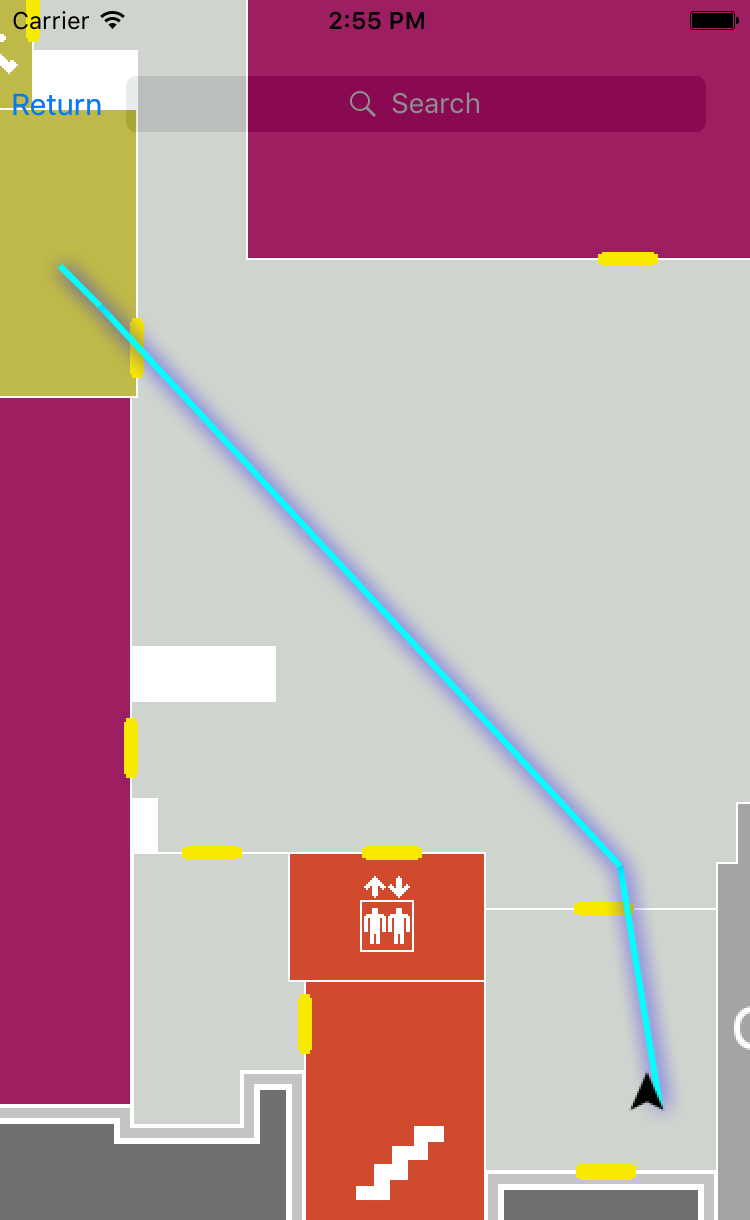
\includegraphics[width=0.5\textwidth]{images/smoothPath.png}
\caption{Path displayed without path smoothing.}
\label{fig:smoothPath}
\end{figure}


\end{document}
